\documentclass[11pt,a4paper]{article}

% ---------- Packages ----------
\usepackage[utf8]{inputenc}
\usepackage[T1]{fontenc}
\usepackage{lmodern}
\usepackage{amsmath,amssymb}
\usepackage{enumitem}
\usepackage{geometry}
\usepackage{fancyhdr}
\usepackage[most]{tcolorbox}   % enhanced, breakable
\usepackage{hyperref}

% ---------- Geometry ----------
\geometry{margin=2.5cm}

% ---------- Header/Footer ----------
\setlength{\headheight}{14pt}  % fancyhdr warning verhindern
\pagestyle{fancy}
\fancyhf{}
\lhead{Introduction to Electrical Engineering}
\rhead{Winter Term 2025}
\cfoot{\thepage}

% ---------- Exercise Environment ----------
\newcounter{exercise}
\newenvironment{exercise}[1][]
  {\refstepcounter{exercise}%
   \begin{tcolorbox}[enhanced, breakable, width=\textwidth,
     colback=blue!5!white,colframe=blue!60!black,
     fonttitle=\bfseries\large,
     title=Exercise~\theexercise:~#1]}
  {\end{tcolorbox}}

% ---------- Solution Environment ----------
\newif\ifshowsolutions
\showsolutionstrue  % comment to hide solutions

\newenvironment{solution}
  {\ifshowsolutions
     \begin{tcolorbox}[enhanced, breakable, width=\textwidth,
       colback=green!5!white,colframe=green!50!black,
       fonttitle=\bfseries\large,
       title=Solution]}
  {\end{tcolorbox}\fi}

% ---------- Document ----------
\begin{document}

% ----- Header Box -----
\begin{tcolorbox}[enhanced, breakable, colback=gray!10!white,
  colframe=gray!70!black, fonttitle=\bfseries\large,
  title={Exercise Sheet \#8}: AC Networks, sharp corners, width=\textwidth]
\begin{center}
  Discussion: Dec 8, 2025
\end{center}
\end{tcolorbox}
\vspace{1cm}

% ----- Exercise 1 -----
\begin{exercise}[AC Circuit Analysis]
Find $v(t)$ in the $RLC$ circuit below.

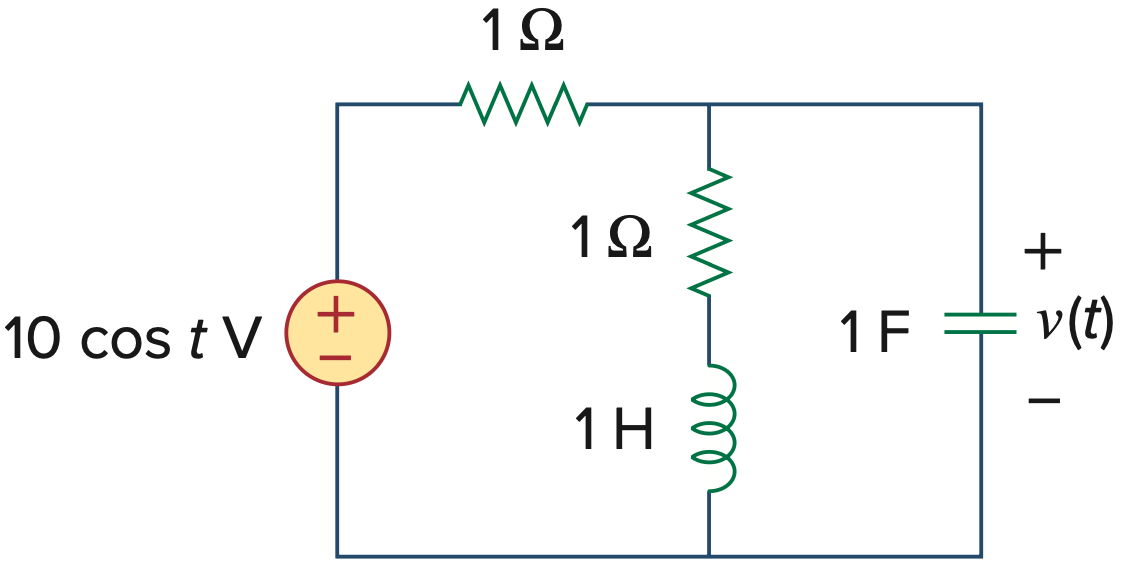
\includegraphics[width=0.7\textwidth]{figures/ACcircuit1.png}
\end{exercise}

\ifshowsolutions
\begin{solution}
We are given the time-domain source
\[
v_s(t) = 10\cos t\,\text{V}.
\]
In complex (exponential) representation we write this as the real part of a complex exponential:
\[
v_s(t) = Re(\underline{\hat{v}}_s e^{j\omega t}),\qquad \underline{\hat{v}}_s = 10,\ \omega=1\ \text{rad/s},
\]
so \(v_s(t)=Re(10 e^{j t})\).

At \(\omega=1\),
\[
\underline{Z}_{R_1} = 1,\qquad \underline{Z}_{R_2} = 1,\qquad \underline{Z}_L = j\omega L = j,\qquad \underline{Z}_C = \frac{1}{j\omega C} = -j.
\]

The series \(R_2\!-\!L\) branch impedance is
\[
\underline{Z}_{RL}=1+j.
\]

The parallel combination of \(\underline{Z}_{RL}\) and \(\underline{Z}_C\) has admittance
\[
\underline{Y}_{p} = \frac{1}{\underline{Z}_{RL}} + \frac{1}{\underline{Z}_C} = \frac{1}{1+j} + \frac{1}{-j}.
\]
Compute each term explicitly:
\[
\frac{1}{1+j} = \frac{1-j}{(1+j)(1-j)} = \frac{1-j}{2} = \tfrac12 - \tfrac12 j,
\qquad
\frac{1}{-j} = j.
\]
Thus
\[
\underline{Y}_p = \left(\tfrac12 - \tfrac12 j\right) + j = \tfrac12 + \tfrac12 j.
\]
Therefore the equivalent impedance of the parallel network is
\[
\underline{Z}_p = \frac{1}{\underline{Y}_p} = \frac{1}{\tfrac12 + \tfrac12 j} = \frac{\tfrac12 - \tfrac12 j}{(\tfrac12)^2 + (\tfrac12)^2} = 1-j.
\]

The total series impedance seen by the source is
\[
\underline{Z}_{\text{tot}} = \underline{Z}_{R_1} + \underline{Z}_p = 1+(1-j) = 2-j.
\]

Now form the complex current \(\underline{\hat{i}}\) (the complex amplitude multiplying \(e^{j t}\)) by dividing the complex source amplitude by the complex impedance:
\[
\underline{\hat{i}} = \frac{\underline{\hat{v}}_s}{\underline{Z}_{\text{tot}}} = \frac{10}{2-j}.
\]
Perform the algebraic division by multiplying numerator and denominator by the conjugate:
\[
\underline{\hat{i}} = 10\frac{2+j}{(2-j)(2+j)} = 10\frac{2+j}{5} = 4+2j.
\]
Thus the complex current amplitude is \(\underline{\hat{i}} = 4+2j\). (Its magnitude is \(|\underline{\hat{i}}| = \sqrt{4^2+2^2} \approx 4.472\) and its angle \(\arg(\underline{\hat{i}}) = \arctan(2/4) = 26.57^\circ\), if one prefers polar form.)

The complex voltage across the parallel network (and thus across the capacitor) is
\[
\underline{\hat{v}}_p = \underline{\hat{i}}\,\underline{Z}_p = (4+2j)(1-j).
\]
Multiply out:
\[
\underline{\hat{v}}_p = 4(1-j)+2j(1-j) = 4-4j+2j-2j^2 = 4-2j+2 = 6-2j.
\]
So the complex amplitude of the capacitor voltage is \(\underline{\hat{v}}_p = 6-2j\).

We may express this two ways:

\textbf{(a) Time-domain real part of the exponential:}
\[
v(t) = Re(\underline{\hat{v}}_p e^{j t}) = Re((6-2j)e^{j t}).
\]
Expanding \((6-2j)e^{jt} = (6-2j)(\cos t + j\sin t)\) and taking the real part gives
\[
v(t) = 6\cos t + 2\sin t.
\]

\textbf{(b) Amplitude–phase form:} compute magnitude and angle of \(\underline{\hat{v}}_p\):
\[
|\underline{\hat{v}}_p| = \sqrt{6^2+(-2)^2} \approx 6.325,
\]
\[
\arg(\underline{\hat{v}}_p) = \arctan\!\bigg(\frac{-2}{6}\bigg) \approx -18.43^\circ.
\]
Thus
\[
\underline{\hat{v}}_p = 6.325\angle(-18.43^\circ),
\]
and therefore
\[
v(t) = 6.325\cos\big(t-18.43^\circ\big)\,\text{V},
\]
which is algebraically equivalent to \(v(t) = 6\cos t+2\sin t\).
\end{solution}
\fi

% ----- Exercise 2 -----
\begin{exercise}[Phase-shifted Source Current]
Determine the value of $i_s(t)$ in the circuit below.

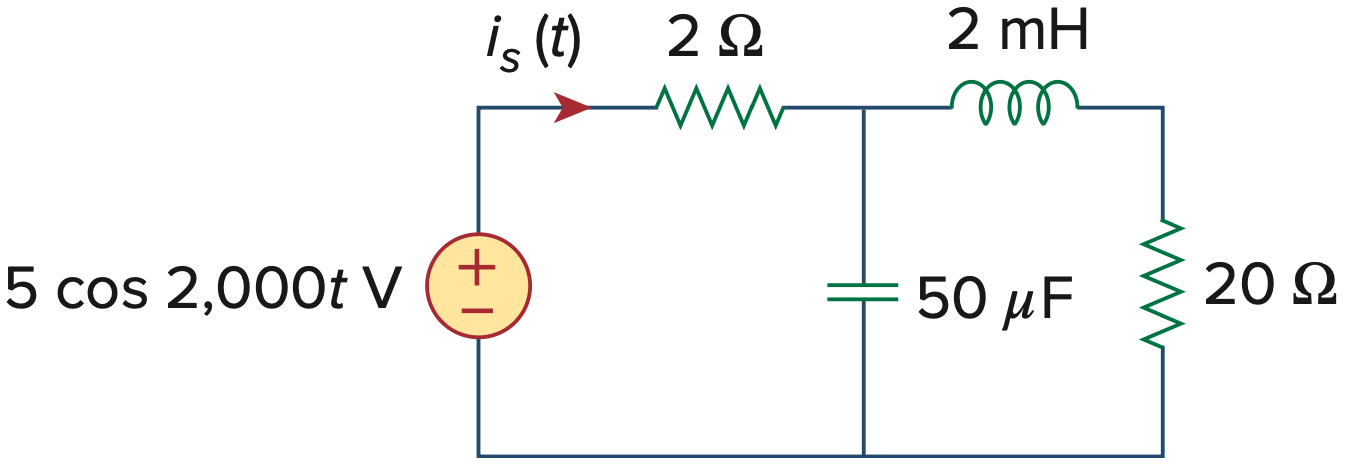
\includegraphics[width=0.7\textwidth]{figures/ACcircuit2.png}
\end{exercise}

\ifshowsolutions
\begin{solution}
\[
\omega = 2000\;\text{rad/s}
\]

\[
\underline{Z}_C = \frac{1}{j \omega C} = \frac{-j}{2000 \cdot 50 \times 10^{-6}}\,\Omega = -j 10\,\Omega
\]

\[
\underline{Z}_{RL} = 20 + j \omega L = (20 + j 2000 \cdot 2 \times 10^{-3})\,\Omega = (20 + j 4)\,\Omega
\]

\[
\underline{Y}_p = \frac{1}{\underline{Z}_C} + \frac{1}{Z_{RL}} = j 0.1 + \frac{1}{20 + j 4} = j 0.1 + \frac{20 - j 4}{416} = \left(\frac{20}{416} + j \frac{37.6}{416}\right)\,\text{S}
\]

\[
\underline{Z}_p = \frac{1}{\underline{Y}_p} = \left(\frac{\frac{20}{416} - j \frac{37.6}{416}}{(\frac{20}{416})^2 + (\frac{37.6}{416})^2}\right)\,\Omega = (4.58716 - j 8.62385)\,\Omega
\]

\[
\underline{Z}_{\text{tot}} = \underline{Z}_{R_2} + Z_p = 2\,\Omega + (4.58716 - j8.62385)\,\Omega = (6.58716 - j 8.62385)\,\Omega
\]

\[
\underline{\hat{i}}_s = \frac{\underline{\hat{v}}_s}{\underline{Z}_{\text{tot}}} = \frac{5}{6.58716 - j 8.62385}\,\text{A} = (0.27714 + j 0.36949)\,\text{A}
\]

\[
\hat{i}_s = \sqrt{(0.27714)^2 + (0.36949)^2}\,\text{A} = 0.460753\,\text{A}
\]

\[
\varphi_{i_s} = \tan^{-1}\!\left(\frac{0.36949}{0.27714}\right) = 52.6263^\circ
\]

\[
i_s(t) = 460.7 \cos\!\left(2000t + 52.63^\circ\right)\,\text{mA}
\]
\end{solution}
\fi

% ----- Exercise 3 -----
\begin{exercise}[Equivalent Impedance]
Find $\underline{Z}_{eq}$ in the circuit below.

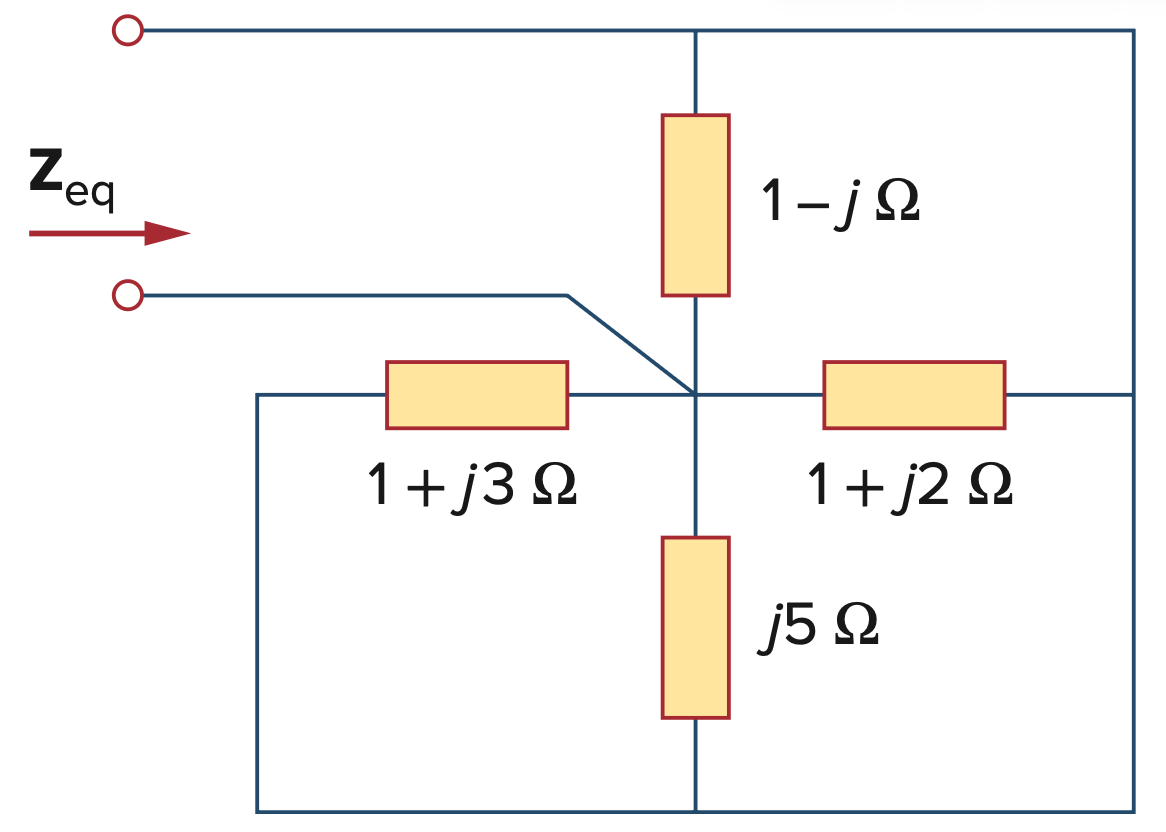
\includegraphics[width=0.7\textwidth]{figures/ACcircuit3.png}
\end{exercise}

\ifshowsolutions
\begin{solution}
\[
\underline{Y} = \frac{1}{\underline{Z}_1} + \frac{1}{\underline{Z}_2} + \frac{1}{\underline{Z}_3} + \frac{1}{\underline{Z}_4} = \frac{1}{1 - j} + \frac{1}{1 + j 2} + \frac{1}{1 + j 3} + \frac{1}{j 5}
\]
\[
= \frac{1 + j}{2} + \frac{1 - j 2}{5} + \frac{1 - j 3}{10} + \frac{-j 5}{25} = \frac{25 + 10 + 5 + j (25 - 20 - 15 - 10)}{50} = (0.8 - j 0.4)\,\text{S}
\]

\[
\underline{Z}_{eq} = \frac{1}{\underline{Y}} = \frac{1}{0.8 - j 0.4} = \frac{0.8 + j 0.4}{0.8^2 + 0.4^2} = (1 + j 0.5)\,\Omega
\]
\end{solution}
\fi

% ----- Exercise 4 -----
\begin{exercise}[Stepwise Voltage Division]
\begin{enumerate}[label=\alph*)]
  \item Calculate the phase shift of the circuit below.
  \item State whether the phase shift is leading or lagging (output with respect to input).
  \item Determine the magnitude of the output when the input is $120\,\text{V}$.
\end{enumerate}

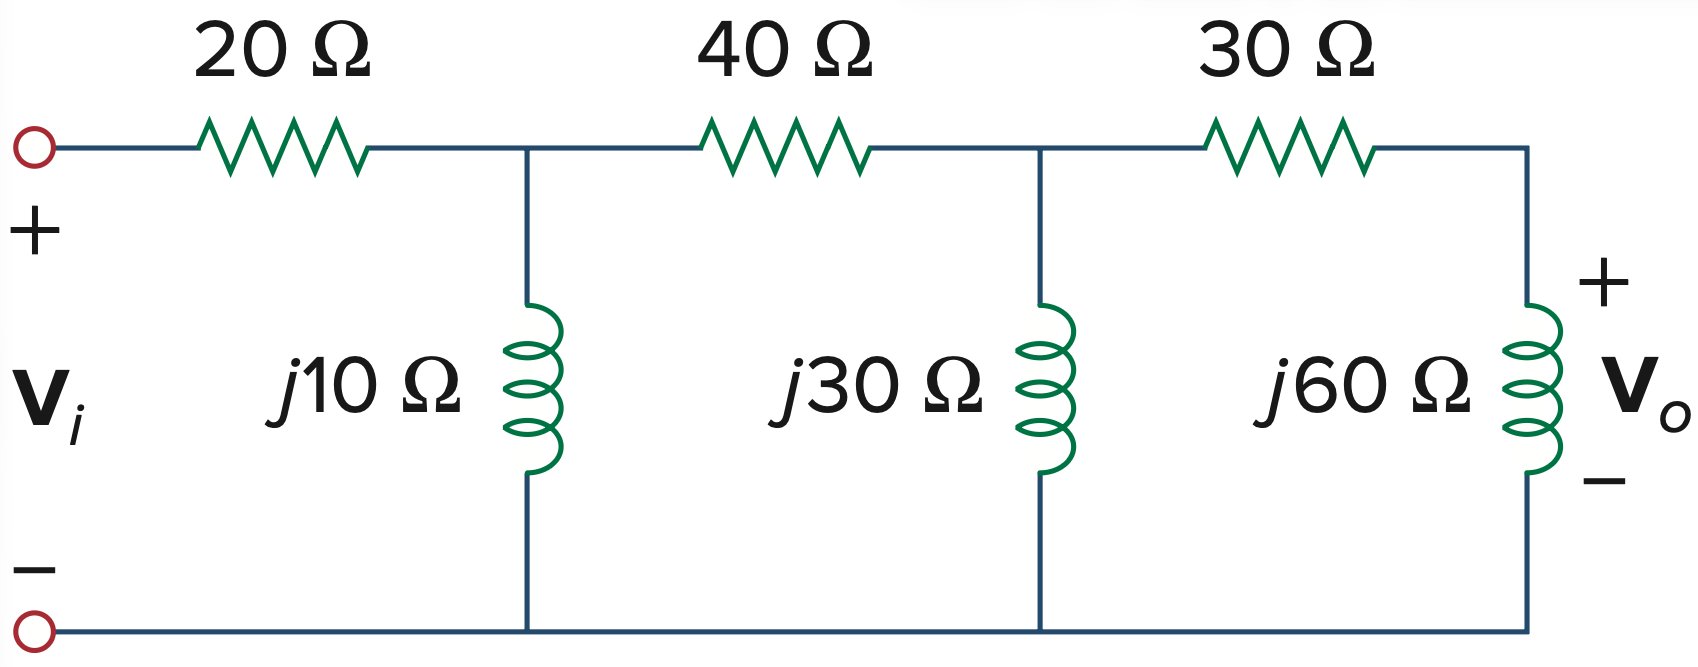
\includegraphics[width=0.7\textwidth]{figures/ACcircuit4.png}
\end{exercise}

\ifshowsolutions
\begin{solution}
\begin{enumerate}[label=\alph*)]
\item We take the input \(\underline{v}_i\) as the reference phasor (angle \(0^\circ\)) and denote the node voltages by \(\underline{v_1}, \underline{v}_2, \underline{v}_3\) (with \(\underline{v}_3 = \underline{v}_o\)).

Step 1: Relation between $\underline{v}_3$ and $\underline{v}_2$

Node 3 is a simple divider between the series resistor \(R_3\) and the inductor \(\underline{Z}_3\):
\[
\underline{v}_3 = \underline{v}_2 \cdot \frac{\underline{Z}_3}{R_3 + \underline{Z}_3}.
\]
With \(R_3 = 30,\; \underline{Z}_3 = j60\):
\[
\frac{\underline{v}_3}{\underline{v}_2} = \frac{j60}{30 + j60} = \frac{1}{1 - j 0.5} = 0.8 + 0.4\,j
\]
\[
= \sqrt{0.8^2 + 0.4^2} \cdot \exp\!\left(j \arctan\!\left(\frac{0.4}{0.8}\right)\right) = 0.894427 \cdot \exp(j 26.565^\circ).
\]

Step 2: Equivalent impedance seen from node 2

Node 2 sees \(\underline{Z}_2\) in parallel with the series path \(R_3 + \underline{Z}_3\):
\[
\underline{Z}_{\text{eq2}} = \frac{\underline{Z}_2 (R_3 + \underline{Z}_3)}{\underline{Z}_2 + (R_3 + \underline{Z}_3)}.
\]
With \(\underline{Z}_2 = j30\):
\[
R_3 + \underline{Z}_3 = 30 + j60,
\]
\[
\underline{Z}_{\text{eq2}} = \frac{j30 (30 + j60)}{j30 + (30 + j60)} = \frac{j900 - 1800}{30 + j90} = \frac{27000 + j189000}{9000} = 3 + j21.
\]

Now apply the divider between \(R_2\) and \(\underline{Z}_{\text{eq2}}\):
\[
\underline{v}_2 = \underline{v}_1 \cdot \frac{\underline{Z}_{\text{eq2}}}{R_2 + \underline{Z}_{\text{eq2}}}.
\]
\[
\frac{\underline{v}_2}{\underline{v}_1} = \frac{3 + j21}{40 + 3 + j21} = \frac{(3 + j21) (43 - j21)}{43^2 + 21^2} = \frac{57 + j84}{229}
\]
\[
= \frac{\sqrt{57^2 + 84^2}}{229} \cdot \exp\!\left(j \arctan\!\left(\frac{84}{57}\right)\right) = 0.443291 \cdot \exp\!\left(j 55.840^\circ\right).
\]

Step 3: Equivalent impedance seen from node 1

Node 1 sees \(\underline{Z}_1\) in parallel with the series path \(R_2 + \underline{Z}_{\text{eq2}}\):
\[
\underline{Z}_{\text{eq1}} = \frac{\underline{Z}_1 (R_2 + \underline{Z}_{\text{eq2}})}{\underline{Z}_1 + (R_2 + \underline{Z}_{\text{eq2}})}
\]

\[
R_2 + \underline{Z}_{\text{eq2}} = 40 + 3 + j21 = 43 + j21,
\]
\[
\underline{Z}_1 (R_2 + \underline{Z}_{\text{eq2}}) = j10 (43 + j21) = -210 + j430
\]
\[
\underline{Z}_1 + (R_2 + \underline{Z}_{\text{eq2}}) = j10 + (43 + j21) = 43 + j31
\]
Thus
\[
\underline{Z}_{\text{eq1}} = \frac{-210 + j430}{43 + j31} = \frac{(-210 + j430)(43 - j31)}{43^2 + 31^2} = \frac{4300 + j25000}{2810}
\]
\[
= \sqrt(4300^2 + 25000^2) \cdot \exp\!\left(j \arctan\!\left(25000/4300\right)\right) \cdot \frac{1}{2810} = 9.027439 \cdot \exp\!\left(j 80.241^\circ\right).
\]

Then the divider between \(R_1\) and \(\underline{Z}_{\text{eq1}}\) gives:
\[
\underline{v}_1 = \underline{v}_i \cdot \frac{\underline{Z}_{\text{eq1}}}{R_1 + \underline{Z}_{\text{eq1}}}.
\]
\[
R_1 + \underline{Z}_{\text{eq1}} = 20 + \frac{4300 + j25000}{2810} = \frac{20 \cdot 2810 + 4300 + j25000}{2810} = \frac{60500 + j25000}{2810}
\]
\[
= \sqrt(60500^2 + 25000^2) \cdot \exp\!\left(j \arctan\!\left(25000/60500\right)\right) \cdot \frac{1}{2810} = 23.296022 \cdot \exp\!\left(j 22.452^\circ\right)
\]
\[
\frac{\underline{v}_1}{\underline{v}_i} = \frac{9.027439}{23.296022} \cdot \exp\!\left(j (80.241^\circ - 22.452^\circ)\right) = 0.387510 \cdot \exp\!\left(j 57.789^\circ\right)
\]

Step 4: Combine the three ratios

Output relative to input:
\[
\frac{\underline{v}_o}{\underline{v}_i} = \frac{\underline{v}_3}{\underline{v}_i} = \frac{\underline{v}_3}{\underline{v}_2} \cdot\frac{\underline{v}_2}{\underline{v}_1} \cdot\frac{\underline{v}_1}{\underline{v}_i}
\]
\[
= 0.894427 \cdot \exp\!\left(j 26.565^\circ\right) \cdot 0.443291 \cdot \exp\!\left(j 55.840^\circ\right) \cdot 0.387510 \cdot \exp\!\left(j 57.789^\circ\right)
\]
\[
= 0.153644 \cdot \exp\!\left(j 140.194^\circ\right)
\]
\[
\Rightarrow \varphi = 140.2^\circ
\]

\item Since the phase shift is positive (\(+140.2^\circ\)), the output phasor **leads** the input phasor.

\item Magnitude of the output when \(V_i = 120\,\text{V}\):
\[
V_o = 0.153644 \cdot 120\,\text{V} \approx 18.44\,\text{V}
\]
\end{enumerate}
\end{solution}
\fi

% ----- Exercise 5 -----
\begin{exercise}[Nodal Analysis]
Determine $i$ in the circuit below.

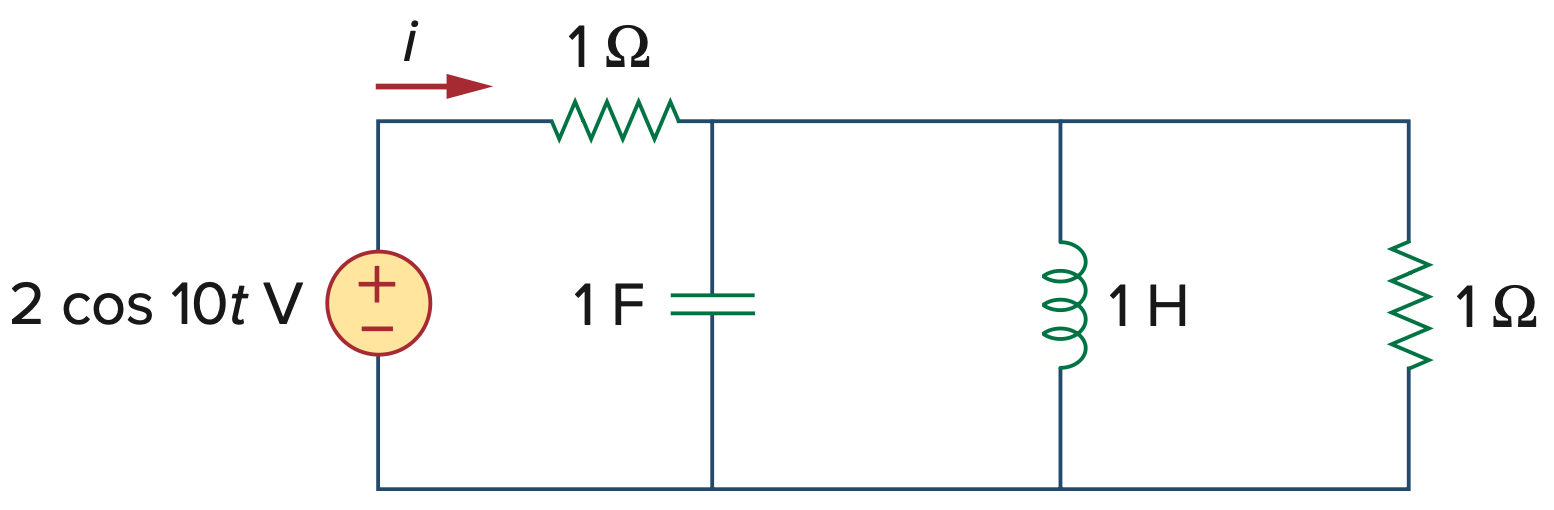
\includegraphics[width=0.7\textwidth]{figures/ACnodal.png}
\end{exercise}

\ifshowsolutions
\begin{solution}
\[
v_s(t) = 2\cos(10t)\quad\Rightarrow\quad \omega=10
\]
Capacitor and inductor admittances (1\,F and 1\,H):
\[
\underline{Y}_C = j\omega C = j10,\qquad \underline{Y}_L = \frac{1}{j\omega L} = -\frac{j}{10} = -j0.1,
\]
and the parallel resistor gives \(R = 1\). Thus the total admittance of the parallel block is
\[
\underline{Y} = R + \underline{Y}_C + \underline{Y}_L = 1 + j10 - j0.1 = 1 + j9.9.
\]

KCL at the node (current through series \(1\Omega\) equals current into the parallel block):
\[
\frac{\hat{v}_s - \underline{\hat{v}}}{1} = \underline{\hat{v}}\;\underline{Y}
\quad\Longrightarrow\quad
\underline{\hat{v}}\,(1 + \underline{Y}) = \hat{v}_s
\quad\Longrightarrow\quad
\underline{\hat{v}} = \frac{\hat{v}_s}{1 + \underline{Y}}.
\]
The source current \( \underline{\hat{i}}\) (which is \(i\) in time domain) is the current through the series \(1\Omega\):
\[
\underline{\hat{i}} = \frac{\hat{v}_s - \underline{\hat{v}}}{1} = \hat{v}_s \frac{\underline{Y}}{1 + \underline{Y}}
\]

Substitute \(\underline{Y} = 1 + j9.9\):
\[
\underline{\hat{i}} = 2 \cdot \frac{1 + j9.9}{2 + j9.9} = \frac{200.02 + j19.8}{102.01} \approx (1.9608 + j0.1941)\,\text{A}
\]

Magnitude, phase and back to the time domain (cosine reference):
\[
i(t) = 1.9704\cos\big(10t + 5.655^\circ\big)\,\text{A}
\]
\end{solution}
\fi

\end{document}